\chapter{Extending A Genetic Algorithm Model To The Diploid Case} \label{ch:GA model Diploid}

This chapter describes a simple Markov model for evolution under the
influence of crossing over and mutation; it is a non-overlapping,
generational, infinite population model under the assumption of {\em complete panmixia} (random mating) and no
selective pressure. This chapter contributes to the elegance and
simplicity of the abstract development and manifests diploid evolution equations can be represented by haploid equations.

A basic syntactic model for haploid and diploid genomes is considered in the beginning and commented on its expressive power. Then the mechanics of how the $(n+1)$th generation is obtained from the $n$th generation are
defined abstractly in procedural terms, which serves to motivate the equations governing evolution.

Next evolution equations are developed corresponding to the
procedural description defining evolution for a population of
diploid genomes. Observations concerning the form and symmetry of
those equations directly lead to decoupling from the diploid case a
haploid model sufficient to determine evolutionary trajectories for
the diploid case.    

\section{Model} \label{Model}
A haploid genome $g$ is defined syntactically as a length $\ell$
binary string.  A collection of $h$ chromosomes may be modeled by
partitioning $g$ into $h$ segments (of arbitrary lengths $\ell_1,
\ldots , \ell_h$; thus $\ell = \ell_1 + \cdots + \ell_h$).
Partitioning may be extended to chromosomes so as to interpret each as
a collection of genes.  If continued to the granularity of pairs of
bits, partitioning allows, for example, representing the four
possibilities Adenine, Guanine, Cytosine, and Thymine.

A diploid genome $\alpha = \langle \alpha_0, \alpha_1 \rangle$ is
likewise defined syntactically as a pair of length $\ell$ binary
strings.  Although simple, that syntax is flexible and possesses
significant modeling power by means of tailoring partitioning to
application.  We concentrate on the abstract level, considering the
evolution of a non-overlapping, generational, infinite population
model assuming panmixia and no selective pressure. We are not concerned with 
whether and how partitioning is defined as it is irrelevant 
to the development.

Following Hardy (see \cite{Hardy1908}), the model $q^{n}$ at generation $n$
is a vector having for component $q_\alpha^n$ the prevalence of
diploid $\alpha\,$ (the probability of selecting $\alpha$ \nudge at
generation $n$, assuming unbiased selection).\footnote{The
  representation here is the conceptual equivalent of Hardy's model.}
Ordered diploid $\gamma = \langle \gamma_0, \gamma_1 \rangle$ is
produced for generation $n+1$ according to following procedural
description.

  Assuming independent selection events:
\begin{itemize}
\item From parent $\alpha$ --- selected with probability
  $q_\alpha^n$ --- obtain gamete $\gamma_0$
\item From parent $\beta$ --- selected with probability $q_\beta^n$
  --- obtain gamete $\gamma_1$
\end{itemize}
Following Gieringer (see \cite{Geiringer1944}), let the transmission
function $t_\alpha(g)$ be the probability that gamete $g$ is produced
from parental genome $\alpha$.  It follows from the above that the
equation determining the next generation $q^{n+1}$ is
\begin{equation}
\label{model0}
q_\gamma^{n+1} \; = \;
\sum_{\alpha} \, q_\alpha^n \, t_\alpha(\gamma_0) 
\sum_{\beta} \,q_\beta^n \, t_\beta(\gamma_1)\\[-.05in]
\end{equation}

It should be appreciated that the Mendelian (see \cite{Mendel1866}) laws of
segregation\footnote{Alleles of a given locus segregate into separate
  gametes.} and independent assortment\footnote{Alleles of one gene
  sort into gametes independently of the alleles of another gene.}
need not be respected by the transmission function.


The right hand side of (\ref{model0}) is invariant under interchange
of the summation variables $\alpha$ and $\beta$, which is equivalent
to interchanging $\gamma_0$ and $\gamma_1$.  This symmetry reflects
the fact that which haploid of $\gamma$ is designated as $\gamma_0$ is
arbitrary,\\[-.05in]
\[
q_{\langle \gamma_0, \gamma_1 \rangle}^{n+1} \; = \;
q_{\langle \gamma_1, \gamma_0 \rangle}^{n+1}\\[.1in]
\]
The model corresponding to (\ref{model0}) is low-level in the sense
that it regards $\langle \gamma_0, \gamma_1 \rangle$ and $\langle
\gamma_1, \gamma_0 \rangle$ as distinct when $\gamma_1 \neq \gamma_0$.
A higher-level model based on sets is easily obtained,
\[
q_{\{\gamma_0, \nudge \gamma_1\}} \; = \; \left\{
\begin{array}{ll}
2 \nudge q_{\langle \gamma_0, \gamma_1 \rangle} & \mbox{ if $\gamma_0 \neq \gamma_1$}\\
\phantom{2 \nudge }q_{\langle \gamma_0, \gamma_1 \rangle} & \mbox{ otherwise}
\end{array}
\right.\\[.05in]
\]
which is in agreement with Hardy (see \cite{Hardy1908}) (issues he considered
and results he obtained relating to invariant distributions for a
particular sort of transmission function are not here mentioned
because they are irrelevant to the purpose of this section).

\section{Reduction}

Evolution equation (\ref{model0}) may be reduced to the haploid case.
Its right hand side is the product of two summations; denote the first
by $p_{\gamma_0}^{n+1}$ and the second by $p_{\gamma_1}^{n+1}$ so that
\begin{equation}
\label{model1}
q_{\langle \gamma_0, \gamma_1 \rangle}^{n+1} \; = \;
p_{\gamma_0}^{n+1} \, p_{\gamma_1}^{n+1}\\[.05in]
\end{equation}
where for any haploid $\gamma_0$,
\begin{equation}
\label{model00}
p_{\gamma_0}^{n+1} \; = \;
\sum_{\alpha} \,q_\alpha^n \, t_\alpha(\gamma_0)
\end{equation}
It suffices to determine the evolution of the distributions $p^{n}$.
Uncoupling \nudge $p$ \nudge from \nudge $q$ \nudge using
(\ref{model00}), and equation (\ref{model1}) with superscript $n$ ---
instantiate the $n$ in (\ref{model1}) with $n-1$ --- yields the
evolution equation
\begin{eqnarray}
\label{model2}
p_{\gamma_0}^{n+1} & = &
\sum_{\alpha_0, \, \alpha_1} \, q_{\langle \alpha_0, \,\alpha_1 \rangle}^n \,
t_{\langle \alpha_0, \,\alpha_1 \rangle}(\gamma_0) \nonumber \\
& = &
\sum_{\alpha_0, \, \alpha_1} \, p_{\alpha_0}^n \, p_{\alpha_1}^n \,
t_{\langle \alpha_0, \,\alpha_1 \rangle}(\gamma_0) 
\end{eqnarray}
The $p^n$ are in fact distributions; summing equation
(\ref{model1}) with superscript $n$ yields
\[
1 \; = \; \sum_\alpha \, q_\alpha^n \; = \;
\sum_{\alpha_0, \, \alpha_1} \, p_{\alpha_0}^n \, p_{\alpha_1}^n \; = \;
\Big( \sum_{\alpha_0} \, p_{\alpha_0}^n \Big)^2
\]
Let $[\mbox{\em expression\/} ]$ denote $1$ if {\em expression\/} is
true, and $0$ otherwise.\footnote{$[ \cdots ]$ is sometimes referred to
  as an {\em Iverson bracket}.}  The weighted count of haploid
$g$ in generation $n$ is
\begin{eqnarray}
\label{project}
  & &
  \sum_{\alpha_0, \, \alpha_1} \, q_{\langle \alpha_0, \alpha_1 \rangle}^n
([g = \alpha_0] + [g = \alpha_1]) \\ & = &
\sum_{\alpha_0, \, \alpha_1} \, p_{\alpha_0}^n \, p_{\alpha_1}^n [g = \alpha_0] + 
\sum_{\alpha_0, \, \alpha_1} \, p_{\alpha_0}^n \, p_{\alpha_1}^n [g = \alpha_1] \\[0.05in]
& = & 2 \nudge p_g^n
\end{eqnarray}

Hence the (normalized) prevalence of haploid $g$ in generation $n$ is
the $g\,$th component of the distribution $p^n$. \linebreak
Moreover, (\ref{project}) and (\ref{model1}) show (for $n >
0$) invertibility of the map
\[
  \pi \nudge : \nudge {\bm q}^{n} \; \longmapsto \; {\bm p}^{n}
\]

Evolution equation (\ref{model2}) in matrix form is
\begin{equation}
\label{model3}
p_g^\prime \; = \; p^T M_g \,\nudge p
\end{equation}
where current state $p$ (generation $n$) and next state $p^\prime$
(generation $n+1$) are column vectors, and the $g\,$th transmission
matrix is
\begin{equation} \label{Mg}
\Big(M_g \Big)_{u,v} \; = \; t_{\langle u, v \rangle}(g)
\end{equation}
(vectors and matrices are indexed by haploids --- length $\ell$ binary
strings).

\section{Specialization}\label{specialize}
This section summarizes from the development in Vose (see \cite{Vose1999}).
It specializes the haploid evolution equations in the previous section 
to a context where mask-based crossing over and mutation operators are used, 
leading to Vose's infinite population model for Genetic Algorithms.  Whereas 
in previous sections {\em component} referred to a component
of a distribution vector $q^n$ or $p^n$, in this section a component
is either a probability (when when speaking of a component of a
distribution vector), or a bit (when speaking of a component of a
haploid).

The set of haploids (i.e., length $\ell$ binary strings) is a
commutative ring $\mathcal{R}$ under component-wise addition and
multiplication modulo $2$.  This algebraic structure is crucial to
Vose's specialization and subsequent analysis of
(\ref{model3}). Denote the additive identity by ${\bf 0}$ and the
multiplicative identity by ${\bf 1}$, and let $\overline{g}$
abbreviate ${\bf 1} + g$.  Except when explicitly indicated otherwise,
operations acting on elements of $\mathcal{R}$ are as defined in this
paragraph.\footnote{In particular, $g \overline{g} = {\bf 0} = g+g$,
  $g^2 = g$, $g + \overline{g} = {\bf 1}$ for all $g \in
  \mathcal{R}$.}

\section{Mutation}
<<<<<<< HEAD
Mutation simulates effects of error that happen with low probability during duplication of chromosome. 
Mutation provides mechanism to inject new strings into the next generation population which gives {\em RHS} 
ability to search beyond the confines of initial population.

Symbol $\bm{\mu}$ is used to represent mutation distribution describing the probability $\bm{\mu}_i$ with which 
$i \in \Omega$ is selected to be a mutation mask. $\bm{\mu} : \Omega \rightarrow \Omega$ is nondeterministic mutation 
function where the result $\bm{\mu}(x)$ of applying mutation function on $x$ is $x + i$ with probability 
$\bm{\mu}_i$ of distribution $\bm{\mu}$ where $i$ is {\em mutation mask}. Mutating $x$ using mutation mask $i$ 
alters the bits of $x$ in those positions the mutation mask $i$ is 1.
$\bm{\mu} \in [0, 0.5)$ is regarded as a {\em mutation rate} which implicitly specifies distribution $\bm{\mu}$ 
according to rule \cite{VoseWright1998}
=======
Mutation simulates effects of error that happen with low probability during duplication of chromosome. Mutation provides mechanism to inject new strings into the next generation population which gives {\em RHS} ability to search beyond the confines of initial population.

Symbol $\bm{\mu}$ is used to represent mutation distribution describing the probability $\bm{\mu}_i$ with which $i \in \Omega$ is selected to be a mutation mask. $\bm{\mu} : \Omega \rightarrow \Omega$ is nondeterministic mutation function where the result $\bm{\mu}(x)$ of applying mutation function on $x$ is $x + i$ with probability $\bm{\mu}_i$ of distribution $\bm{\mu}$ where $i$ is {\em mutation mask}. Mutating $x$ using mutation mask $i$ alters the bits of $x$ in those positions the mutation mask $i$ is 1.
$\bm{\mu} \in [0, 0.5)$ is regarded as a {\em mutation rate} which implicitly specifies distribution $\bm{\mu}$ according to rule (see \cite{VoseWright1998})
>>>>>>> f3bf8bb1ca6e00c482d1b1f3863823e9ea28d462
\[
\bm{\mu}_i = (\bm{\mu})^{{\bf 1}^Ti} (1-\bm{\mu})^{\ell- {\bf 1}^Ti}
\]
If $g$ should mutate to $g^\prime$ with probability $\rho$,
let\\[-0.2in]
\[
\bm{\mu}_{g + g^\prime} \; = \; \rho\\[0.05in]
\]
Given distribution $\bm{\mu}$, mutation is the stochastic operator sending
$g$ to $g^\prime$ with probability $\bm{\mu}_{g + g^\prime}$.

<<<<<<< HEAD
Mutation considered is {\em independent} for all $j$ and $k$ which means \cite{VoseWright1998}
\[
\bm{\mu}_j = \sum\limits_{k\cdot i=0} \bm{\mu}_{i + j} \sum\limits_{\overline{k} \cdot i=0} \bm{\mu}_{i\cdot j}
\]

=======
>>>>>>> f3bf8bb1ca6e00c482d1b1f3863823e9ea28d462
\section{Crossover}
Crossover refers to crossing over (also termed recombination) between two chromosomes (strings in our case). Crossover like mutation also provides mechanism for injection of new strings into new generation population. Masked based crossover is used in this document. Geiringer (see \cite{Geiringer1944}) used crossover mask with probability (distribution) associated with the mask to generate offsprings from parent chromosomes in absence of mutation and selection. Let $\bm{\chi}_m$ be probability distribution with which $m$ is selected to be a crossover mask.
Following Geiringer (see \cite{Geiringer1944}), if crossing over $u$ and $v$ should produce $u^\prime$ and $v^\prime$ with probability $\rho$, let
\[
\bm{\chi}_m \; = \; \rho
\]
where $m$ is $1$ at components which $u^\prime$ inherits from $u$, and
$0$ at components inherited from $v$.  It follows that\\[-0.3in]
\begin{eqnarray*}
u^\prime & = & m \nudge u + \overline{m} \nudge\nudge v \\
v^\prime & = & m \nudge v + \overline{m} \nudge\nudge u
\end{eqnarray*}
Given distribution $\bm{\chi}$, crossover is the stochastic operator which
sends $u$ and $v$ to $u^\prime$ and $v^\prime$ with probability $\bm{\chi}_m/2$ for each $u^\prime$ and $v^\prime$.

$\bm{\chi}$ can be considered as a {\em crossover rate} that specifies the distribution $\bm{\chi}$ given by rule (see \cite{VoseWright1998})
\[
  \bm{\chi}_i =\begin{cases}
    \bm{\chi}  c_i & \text{if $i>0$}.\\
    1 - \bm{\chi} + \bm{\chi}  c_0 & \text{if $i = 0$}.
  \end{cases}
\]
where $c \in \Lambda$ is referred to as {\em crossover type}. Classical crossover types include {\em 1-point crossover} and {\em uniform crossover}. For {\em 1-point crossover},
\[
  c_i =\begin{cases}
    1/(\ell - 1) & \text{if $\exists k \in (0, \ell).i = 2^k - 1$}.\\
    0 & \text{otherwise}.
  \end{cases}
\]
and for uniform crossover, $c_i = 2^{-\ell}$.

\section{Mixing Matrix}
The combined action of mutation and crossover is referred to as {\em mixing}.
The {\em mixing matrix\/} $M$ is the transmission matrix corresponding to the 
additive identity of $\mathcal{R}$ is
\[
M \; = \; M_{\bf 0}\\[-0.01in]
\]
Crossover and mutation are defined in a manner respecting arbitrary partioning and arbitrary linkage to preserve the ability to endow abstract syntax with specialized semantics. Groups of loci can mutate and crossover with arbitrarily specified probabilities as disscussed in above sections. For mutation distribution $\bm{\mu}$ and crossover distribution $\bm{\chi}$, then transmission function can be expressed as (see \cite{VoseWright1998})
\begin{equation}
\label{transmission}
t_{\langle u,v \rangle}(g) \; = \;\,
\sum_{i \nudge \in \nudge \mathcal{R}} \, \sum_{j \nudge \in \nudge \mathcal{R}} \,
\sum_{k \nudge \in \nudge \mathcal{R}}
\bm{\mu}_i \nudge \bm{\mu}_j \, \frac{\bm{\chi}_k + \bm{\chi}_{\overline{k}}}{2} \,
[\nudge k (u + i) + \overline{k}(v + j) \, = \, g\nudge]
\end{equation}
Here a child gamete $g$ is produced via mutation and then crossover (which are operators that
commute). 

The mixing matrix $M$ is a fundamental object, because (\ref{transmission}) implies that evolution equation (\ref{model3}) can be expressed in the form
\begin{equation}
\label{model4}
p_g^\prime \; = \; (\sigma_g \nudge p)^T M \, (\sigma_g \nudge p)
\end{equation}
where the permutation matrix $\sigma_g$ is defined by component equations
\[
(\sigma_g)_{u,v} \; = \; [\nudge u+v = g\nudge ]
\]

\section{Walsh Transorm}
The Walsh matrix is defined by
\[
W_{n,t} = N^{-1/2} (-1)^{n t}
\]
where $N^{-1/2}$ is normalization factor and $n t$ is bitwise dot product of binary representation of number n and t.

The matrix is symmetric, i.e.,
\[
W_{n,t} = W_{n,t}
\]
and it has entries satisfying
\[
W_{n, t + k} = N^{1/2} W_{n, t} W_{n, k}
\]

The practical importance of this symmetry is that the transform and inverse represent same mathematical operation, hence simplifying the derivation and application of the transform. With the normalized form, \textit{Walsh matrix} is its own inverse, i.e.,
\[
W = W^{-1}
\]

In the matrix form, given vector $w$ and matrix $A$, let $\widehat{w}$ and
$\widehat{A}$ denote the Walsh transform of $w$ and $A$ respectively. Then $\widehat{w} = Ww$ and
$\widehat{A} = WAW$. If $w$ is a row vector, then $w$ in its Walsh basis $\widehat{w}$ represents $wW$.

Finite discrete Walsh transform pair on N sampling points, $x_t$, can be expressed as (see \cite{Beauchamp1975} )
\begin{equation}
\label{WalshT}
X_n = \sum_{t=0}^{N-1} x_t W_{n,t}
\end{equation}
\[
n = 0, 1, 2...N-1
\]
and
\[
x_t = \sum_{n=0}^{N-1} X_n W_{n,t}
\]
\[
t = 0, 1, 2...N-1
\]

\section{Walsh Transform Adaptation}
The Walsh transform has spectacular ability to unravel the intricacies of mixing. And that is why we adapt Walsh transform methods for computing evolutionary trajectories, which have already been established for Vose's haploid model (see \cite{VoseWright1998}). Adaptation of Walsh transformation efficiently models infinite diploid population evolution. This adaptation of Walsh transormation helps in making feasible comparisons between finite and infinte diploid population short-term evolutionary behavior.
Recalling evolution equation (\ref{model4}), without selection, specialized to Vose's infinite population model expressed in mixing matrix's term,
\[
p_g^\prime \; = \; (\sigma_g \nudge p)^T M \, (\sigma_g \nudge p)
\]
where the permutation matrix $\sigma_g$ is defined by component
equations
\[
(\sigma_g)_{u,v} \; = \; [\nudge u+v = g\nudge ]
\]

In our model, the Walsh matrix $W$
is defined by component equations
\[
W_{u,v} \; = \; 2^{-\ell/2} (-1)^{u^T v}
\]
where the subscripts \nudge u, \nudge v (which belong to $\mathcal{R}$) on the left hand side are interpreted on the right hand side as column vectors in $\mathbb{R}^{\ell}$.
Columns of $W$ form the orthonormal basis --- the
{\em Walsh basis\/} --- which simultaneously diagonalizes the
$\sigma_g$.

A change of basis which simultaneously diagonalizes the $\sigma_g$
unravels the evolution equation (\ref{model4}).  
Expressed in the Walsh basis (see \cite{VoseWright1998}), the mixing matrix
takes the form
\begin{equation}
\label{Mhat}
\widehat{M}_{u,v} \; = \; 2^{\,\ell-1} \,[\nudge u \nudge v = {\bf
    0}\nudge]\, \widehat{\bm{\mu}}_u \nudge \widehat{\bm{\mu}}_v \!  \sum_{k
  \nudge \in \nudge \overline{u+v} \nudge \mathcal{R}} \bm{\chi}_{k + u} +
\bm{\chi}_{k + v}
\end{equation}
and equation (\ref{model4}) takes the form
\begin{equation}
\label{model5}
\widehat{p}_g^{\,\,\prime} \; = \; 2^{\,\ell/2} \sum_{i \nudge \in \nudge g \mathcal{R}}
\widehat{p}_i \, \nudge \widehat{p}_{i+g} \,\widehat{M}_{i,i+g}
\end{equation}
where $g \mathcal{R} = \{g \nudge i \, | \, i \in \mathcal{R} \}$ (for
any $g \in \mathcal{R}$).

The mapping from generation $n$ to generation $n+1$, determined in
natural coordinates by equation (\ref{model3}) in terms of the
transmission function (\ref{Mg}), and given in Walsh coordinates by
equation (\ref{model5}) in terms of the mixing matrix (\ref{Mhat}), is
Markovian; the next state $p^\prime$ depends only upon the current
state $p$.  Let $\mathcal{M}$ represent the mixing transformation,
\begin{equation} \label{mixing_transformation}
p^\prime \; = \; \mathcal{M}(p)
\end{equation}
and let $\mathcal{M}^n(p)$ denote the $n$-fold composition of
$\mathcal{M}$ with itself; thus generation $n+1$ is described by
\[
p^{n+1} \; = \; \mathcal{M}^n(p^1)
\]
where $p^1 = \pi (q^1)$.  We have little to say
about the matrix of the Markov chain corresponding to the mixing
transformation $\mathcal{M}$, because it is uncountable; each state is
a distribution vector $p$ describing a population. However, that is
not an obstacle to computing evolutionary trajectories;
(\ref{mixing_transformation}) can be computed in Walsh coordinates
relatively efficiently via (\ref{Mhat}) and (\ref{model5}).

\section{Fast Walsh Transform}
However, computation of discrete Walsh transform given by equation (\ref{WalshT}) takes $N^2$ operations (addition or subtraction).
An algorithm using matrix factorization techniques is found to perform transformation in $N \log_2 N$ operations.
This algorithm is Fast Walsh transform (FWT). Shanks (see \cite{Shanks1969}) described FWT algorithm which is analogous to 
Cooley-Tukey algorithm (see \cite{CooleyTukey1965}) for fast Fourier transformation.

Here is the pseudocode for FWT:
\begin{algorithm}
\caption{FWT pseudocode}
\label{FWTpseudo}
\begin{algorithmic}[1]
\Procedure{FWT}{}
\State $n = 2^\ell$
\For{$i = 0$ to $n$ }
\State $m = 2^{\ell}/2^i$
\State $z = 2^{\ell}/2^(i+1)$
\State \For{$j = 0 to 2^i$}
\State \For{$k = 0 to z$}
\State $t1 = m*j + k$
\State $t2 = m*j + z +k$
\State $a = X[t1]$
\State $b= X[t2]$
\State $X[t1] = a + b$
\State $X[t2] = a - b$

\EndFor
\EndFor
\EndFor
\EndProcedure
\end{algorithmic}
\end{algorithm}
  
  

% \chapter{Experimental Simulations and Measurements} \label{ch:distance}
% This chapter describes how distance between finite diploid population and infinite population is calculated.
% Then it discusses simplifications in computations made by our evolutionary equations and in distance computation. 
% And it goes on to discuss results from simulations and convergence of finite diploid population short-term behavior 
% to evolutionary behavior predicted by infinite population model.

\section{Distance}
Let vector ${\bm f}$ represent a finite diploid population; component
${\bm f}_\alpha$ is the prevalence of diploid $\alpha$.  Let the
support $S_{\bm f}$ of ${\bm f}$ be the set of diploids occurring in
the population represented by ${\bm f}$,\\[-0.03in]
\[
S_{\bm f} \; = \; \{ \alpha \, | \, {\bm f}_\alpha > 0 \}
\]
Let ${\bm q}$ similarly represent an infinite diploid population (see
section \ref{Model}).  As points in $\mathbb{R}^{2^\ell
  \times 2^\ell}$, the Euclidean distance between ${\bm f}$ and ${\bm
  q}$ is \\[-0.175in]
\[
\|{\bm f} - {\bm q} \hspace{0.005in} \| \; = \;
  {\sum_{\alpha}}^{\frac{1}{2}} ({\bm f}_\alpha-{\bm q}_\alpha)^2\\[-.02in]
\]
Whereas a naive computation of this distance involves ${2^\ell \cdot
  2^\ell}$ terms, leveraging equation (\ref{model1}) can significantly
reduce the number of terms involved.  Note that
\begin{equation} \label{d1}
\|{\bm f} - {\bm q} \hspace{0.005in} \|^2 \; = \;
\sum_{\alpha \notin {S_{\bm f}}} ({\bm f}_\alpha-{\bm q}_\alpha)^2 +
\sum_{\alpha \in {S_{\bm f}}} ({\bm f}_\alpha-{\bm q}_\alpha)^2 \\[-.02in]
\end{equation}
Using equation (\ref{model1}) --- ${\bm q}_\alpha = {\bm p}_{\alpha_0}
\nudge {\bm p}_{\alpha_1}$ (suppressing superscripts to streamline
notation) --- together with the fact that ${\bm f}_\alpha = 0$ in
every term of the first sum above, the first sum reduces to
\begin{eqnarray}
  \sum_{\langle \alpha_0, \nudge \alpha_1 \rangle \nudge \notin
    {S_{\bm f}}} ({\bm p}_{\alpha_0} \nudge {\bm p}_{\alpha_1})^2 & =
  & \sum_{\langle \alpha_0, \nudge \alpha_1 \rangle} ({\bm
    p}_{\alpha_0})^2 \nudge ({\bm p}_{\alpha_1})^2 \, - \sum_{\langle
    \alpha_0, \nudge \alpha_1 \rangle\in {S_{\bm f}}} \big( {\bm
    p}_{\alpha_0}\nudge {\bm p}_{\alpha_1} \big)^2 \nonumber
  \\[0.05in] & = & {\sum_{g}}^2 ({\bm p}_{g})^2 \, - \sum_{\alpha \in
    {S_{\bm f}}} ( {\bm q}_{\alpha})^2
      \label{d2}
\end{eqnarray}
\mbox{ }\\[-.15in]
It follows from (\ref{d1}) and (\ref{d2}) that
\begin{eqnarray}
  \|{\bm f} - {\bm q} \hspace{0.005in} \|^2
  & = & 
      {\sum_{g}}^2 ({\bm p}_{g})^2 \, +
      \sum_{\alpha \in {S_{\bm f}}} ({\bm f}_\alpha-{\bm q}_\alpha)^2 -
      \sum_{\alpha \in {S_{\bm f}}} ( {\bm q}_{\alpha})^2
      \nonumber \\[0.05in]
      & = &
      {\sum_{g}}^2 ({\bm p}_{g})^2 \, +
      \sum_{\alpha \in {S_{\bm f}}} {\bm f}_\alpha ({\bm f}_\alpha- 2 {\bm q}_\alpha) \label{d3}
\end{eqnarray}
\mbox{ }\\[-.1in] which involves $2^\ell + |S_{\bm f}|$ terms,
assuming that  $S_{\bm f}$ is known as a byproduct of computing ${\bm f}$.

(\ref{d3}) computes distance between finite and infinite population efficiently.


\section{Simplification} 
The haploid case simplified by equations (\ref{Mhat}) and (\ref{model5})
are the consequence of specializing to Vose's infinite population model and computing in the Walsh basis. Time switching between the standard basis and the Walsh basis is negligible; the fast Walsh transform (in dimension $n$) has complexity $n \nudge \log n$ \cite{Shanks1969}.

Only one mixing matrix as opposed to $2^\ell$ matrices is needed to compute the next generation; evolution equation (\ref{model5}) references the same matrix for every $g$, whereas evolution equation (\ref{model3}) depends upon a different matrix $M_g$ for each choice of $g$. The matrix is computed by a single sum as opposed to a triple sum; compare equation (\ref{Mhat}) with equation (\ref{transmission}).  Also, the relevant quadratic form is computed with a single sum as opposed to a double sum; computing via (\ref{model5}) is linear time in the size of $g \mathcal{R}$ (for each $g$) as opposed to the quadratic time computation (for each $g$) represented by equation (\ref{model3}).

From a computational standpoint, the best-case scenario is where
recomputation of the matrices mentioned in the previous paragraph is
obviated by sufficient memory.  The reduction from $2^\ell$ matrices
to one matrix helps significantly in that regard. To demonstrate this
advantage in concrete terms, consider genomes of length $\ell = 14$.
Using $2^{14}$ matrices each of which contains $2^{14} \times \nudge
2^{14}$ entries of type \verb@double@ requires $32$ terabytes, whereas
the mixing matrix at $2$ gigabytes fits easily within the memory of a
laptop.  Moreover, for a population size of $N \le 2^{20}$, the
distance computation described in the previous section reduces the
number of terms involved by a factor of
$2^{28}/(2^{14} + 2^{N}) \; > \; 252$.

\section{Convergence}

This section presents a cursory numerical investigation of the
convergence of finite diploid population short-term behaviour to that
of the infinite diploid population model as described in section 2
(the underlying haploid model for the infinite population case is
described in section \ref{Model}).

Equations (\ref{model1}), (\ref{Mhat}),
(\ref{model5}), (\ref{d3}) were employed to illustrate efficient
computation of the distance
\[
d \; = \; \|{\bm f}^n - {\bm q}^n \nudge \|
\]
where ${\bm f}^n$ and ${\bm q}^n$ represent finite and infinite diploid
populations at generation $n \in \{1,2,4,8,16,32,64,128\}$
respectively, beginning from a random initial population (${\bm f}^0 =
{\bm q}^0$). Genome lengths $\ell \in \{4,6,8,10,12,14\}$ and population
sizes $N = 2^i$ for integer $0 \le i \le 20$ were considered.  The
crossover distribution ${\bm \chi}$ corresponds to independent assortment of
bits, and the mutation distribution ${\bm \mu}$ corresponds to independent
bit mutation probability $0.001$,

\[
{\bm \chi}_m \; = \; 2^{-\ell}, \;\;\;\;\; {\bm \mu}_g \; = \; (0.001)^{{\bf 1}^{\rm T}
  g}(0.999)^{\ell - {\bf 1}^{\rm T} g}
\]
(subscripts above on the left hand side of an equality are interpreted
on the right hand side of the equality as column vectors in
$\mathbb{R}^{\ell}$). The finite population case is computed using the
itemized procedural definition given in section \ref{Model}; the transmission
function (\ref{transmission}) corresponds to ${\bm \mu}$ and ${\bm
  \chi}$ above (bits mutate independently and are freely assorted).

\begin{figure}[H]
\begin{center}
\subfloat[$\ell = 4$.]{
\resizebox*{6.5cm}{!}{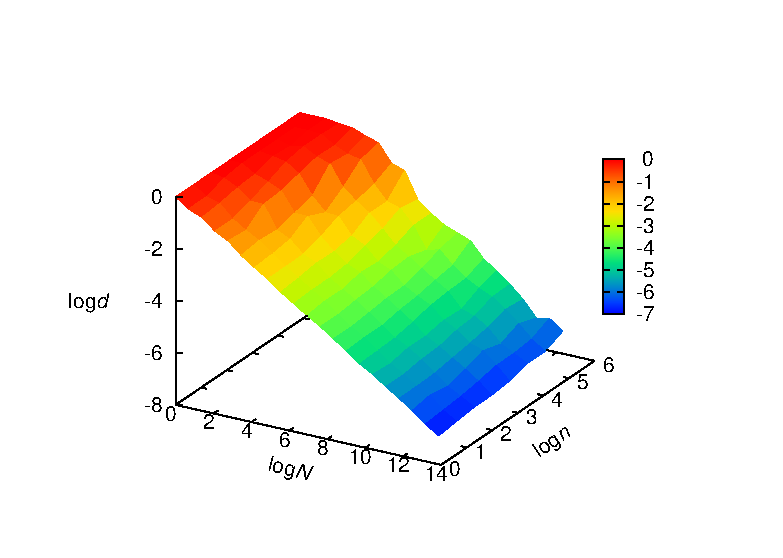
\includegraphics{figures/eps/surf/b4.eps}}}\hspace{5pt}
\subfloat[$\ell = 6$.]{
\resizebox*{6.5cm}{!}{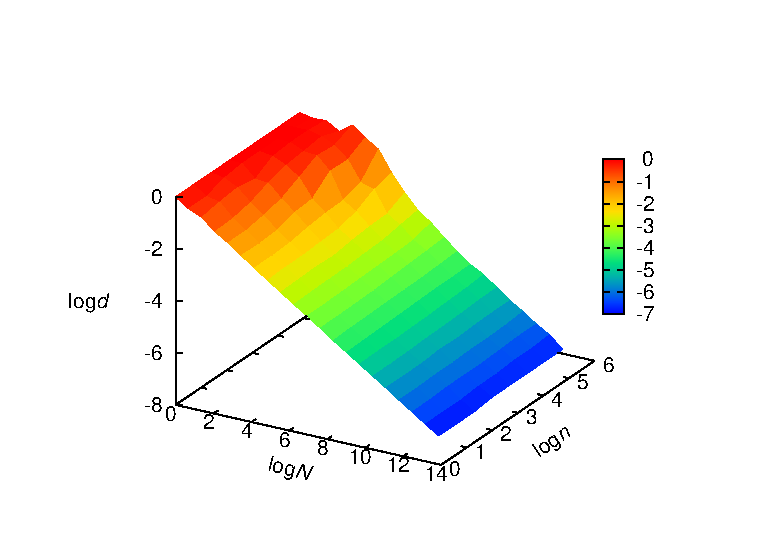
\includegraphics{figures/eps/surf/b6.eps}}}
\end{center}
  
\begin{center}
\subfloat[$\ell = 8$.]{
\resizebox*{6.5cm}{!}{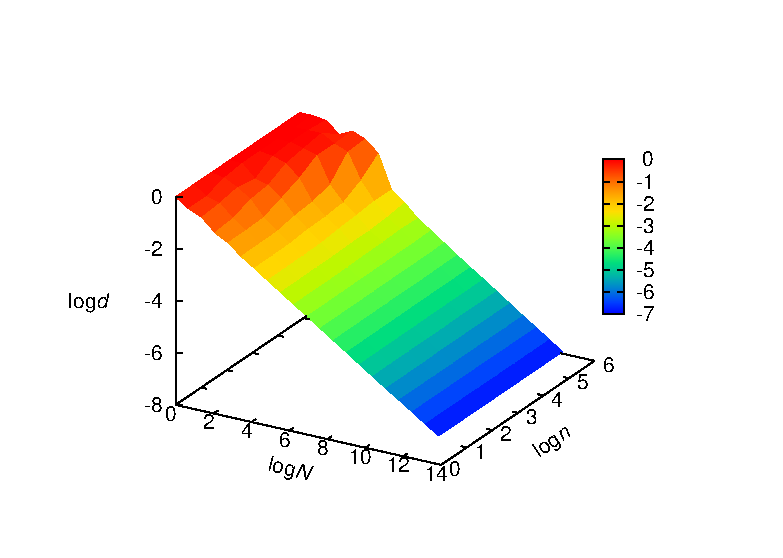
\includegraphics{figures/eps/surf/b8.eps}}}\hspace{5pt}
\subfloat[$\ell = 10$.]{
\resizebox*{6.5cm}{!}{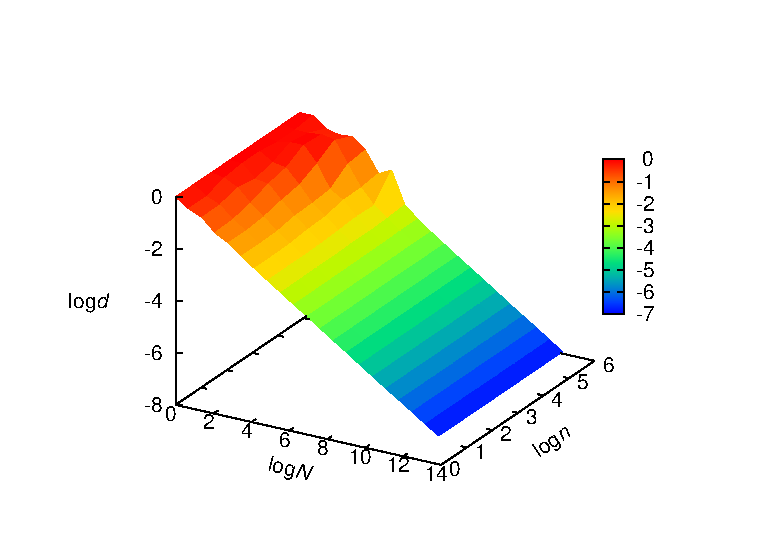
\includegraphics{figures/eps/surf/b10.eps}}}
\end{center}

\begin{center}
\subfloat[$\ell = 12$.]{
\resizebox*{6.5cm}{!}{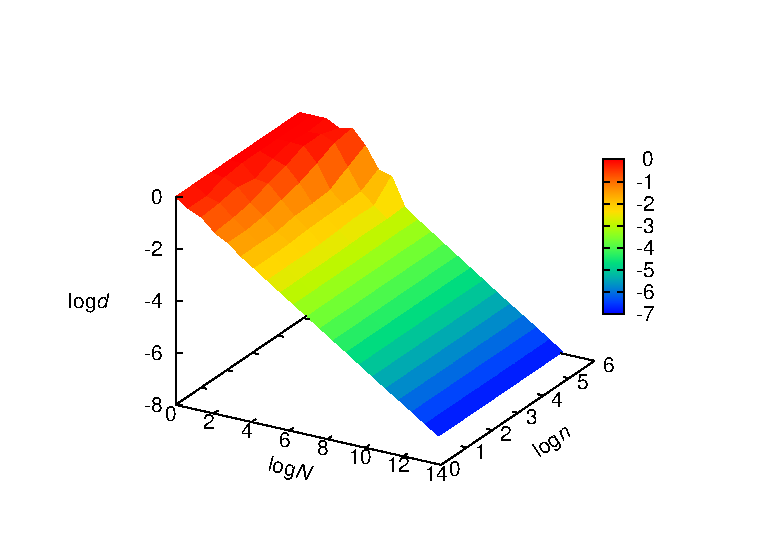
\includegraphics{figures/eps/surf/b12.eps}}}\hspace{5pt}
\subfloat[$\ell = 14$.]{
\resizebox*{6.5cm}{!}{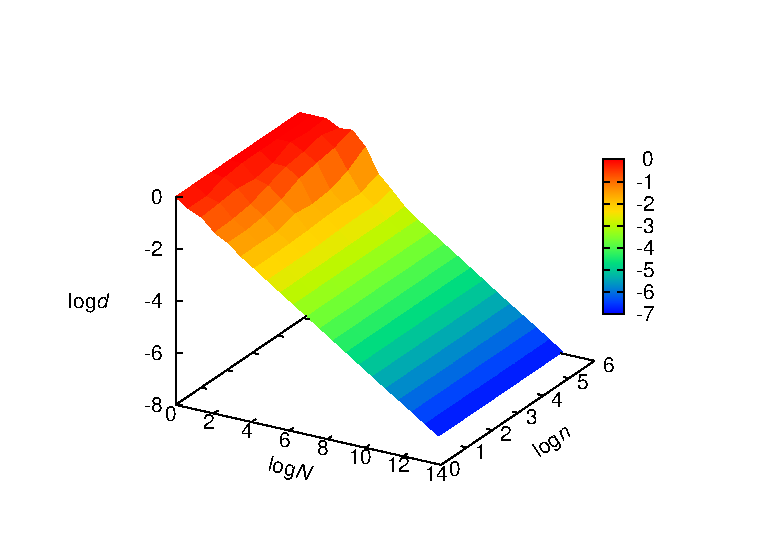
\includegraphics{figures/eps/surf/b14.eps}}}
\caption{\textbf{Convergence of finite population behaviour:} $d$ is
  distance between finite population ${\bm f}^n$ and infinite
  population ${\bm q}^n$ at generation $n$, population size $N$, for
  genome length $\ell$ (bits).}
\label{convergence}
\end{center}
\end{figure}

The data, presented in six surface graphs above and organized by
genome length, shows a near linear dependence of $\log d$ on $\log N$.
As expected, the graphs show smoothing with increasing genome length
(the computation of $d$ involves averaging over $\ell$ components),
and also with increased population size (as explained in
\cite{Vose1999}, the initial transient of a finite haploid population
trajectory converges as $N \rightarrow \infty$ to the corresponding
infinite population model).

%\newpage
  Of particular interest is the linear trend exhibited above.  The
  slope $m$ and intercept $b$ of the regression line
  \begin{equation} \label{regresion}
  \log d = m \log N + b
  \end{equation}
was computed using the data above; each was plotted against genome
length $\ell$ and organized by generation $n$. The resulting
graphs are displayed below.

\begin{figure}[H]
\begin{center}
\subfloat[Slope $m$, genome length $\ell$.]{
\resizebox*{7cm}{!}{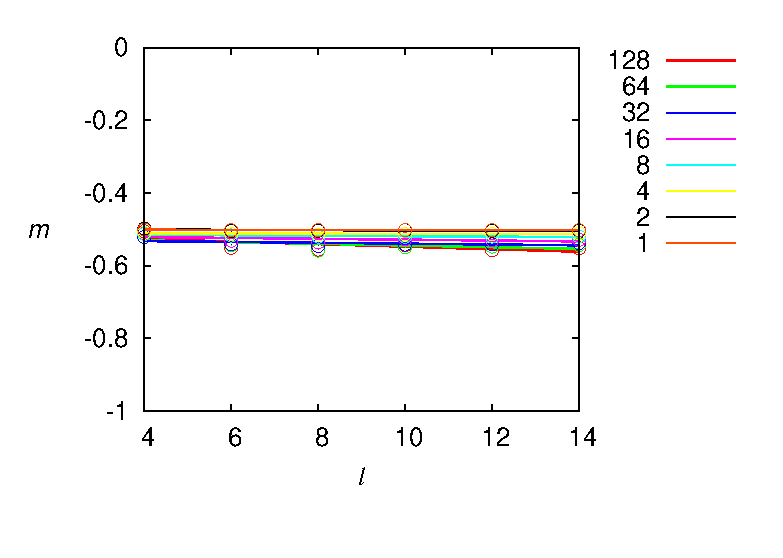
\includegraphics{figures/eps/slope/m.eps}}}\hspace{5pt}
\subfloat[Intercept $b$, genome length $\ell$.]{
\resizebox*{7cm}{!}{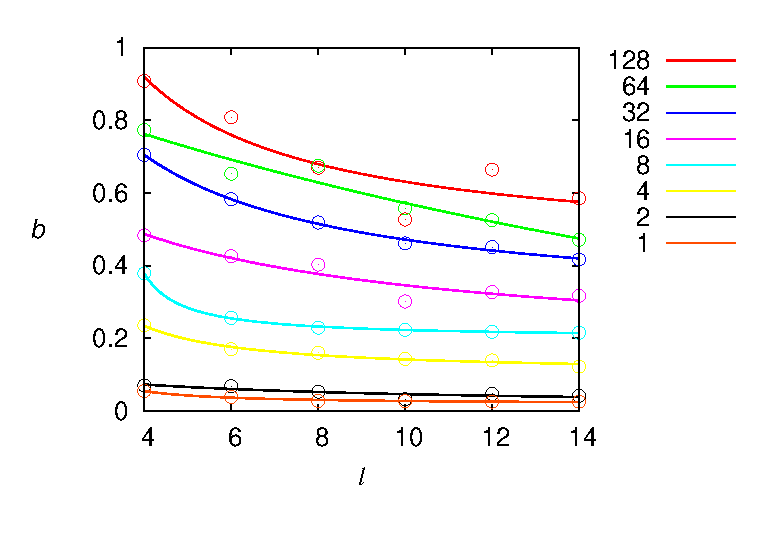
\includegraphics{figures/eps/slope/b.eps}}}
\caption{\textbf{Regression parameters:} multi-plot of slope $m$ and intercept $b$ for generation  $n \in \{1,  2,  4,  8,  16,  32,  64,  128\}$ .}
\label{regression-parameters}
\end{center}
\end{figure}

Taking the exponential of the regression line (\ref{regresion}) yields
the estimate
$d \approx N^m e^b $.

Slopes of the regression lines shown in {\bf Figure \ref{regression-parameters}} are
approximately $-0.5$, indicating
\begin{equation}
\label{covergenceDistance}
d \; \approx \; k/\sqrt{N}.
\end{equation}
 
Vose (see \cite{Vose1999}) calculated variance of next generation population with respect to expected population as 
\[
\mathcal{E}(\| \bm{q} - \mathcal{G}(\bm{p}) \|^2) = (1 - \|\mathcal{G}(\bm{p})\|^2) / \bm{N}
\] 
where $\bm{q}$ is actual population and $\mathcal{G}(\bm{p})$ is expected population.
Let $x$ be the random variable $\| \bm{q} - \mathcal{G}(\bm{p}) \|$. Let $\phi$ be the function $\phi (x) = x^2$ 
which is convex function. Then $\mathcal{E}(\| \bm{q} - \mathcal{G}(\bm{p}) \|^2)$ becomes $\mathcal{E}(\phi (x))$. 
From Jensen's Inequality (see \cite{JensenInequality}),
if $\phi$ is a convex function, then
\begin{eqnarray*}
\phi(\mathcal{E}(x))) & \leq & \mathcal{E}(\phi(x)) \\
\mathcal{E}(x) & \leq & \sqrt{\mathcal{E}(x^2)}
\end{eqnarray*}
Substituting original variables,
\begin{equation}
\label{convergenceRHS}
\mathcal{E}(\| \bm{q} - \mathcal{G}(\bm{p}) \|) \leq \sqrt{(1 - \|\mathcal{G}(\bm{p})\|^2) / \bm{N}}
\end{equation}
Equation \ref{convergenceRHS} shows the expected rate of convergence for the single-step
haploid case; the distance is inversely proportional to square root of population size. 
And equation \ref{covergenceDistance} agrees with  equation \ref{convergenceRHS}.

The consistent convergence rate
across multiple generations is somewhat surprising, simulation
results above indicate it may persist to generation $n = 128$.

The intercept graphs above show the constant of proportionality $k =
e^b$ decreases monotonically with genome length $\ell$, and increases
monotonically with generation $n$.  The increase in $k$ for larger $n$
seems to be a manifestation of the growing nonlinearity uniformly
exhibited by the plots in {\bf Figure \ref{convergence}} as $n$ increases.  It seems
likely that the nonlinearity results from genetic drift experienced by
finite populations (see \cite{CrowKimura}).









